\documentclass[12pt,a4paper]{report}

\usepackage[utf8]{inputenc}
\usepackage[T1]{fontenc}
\usepackage[provide=*,french]{babel}
\usepackage{geometry}
\usepackage{xcolor}
\usepackage{hyperref}
\usepackage{booktabs}
\usepackage{array}
\usepackage{longtable}
\usepackage{enumitem}
\usepackage{fancyhdr}
\usepackage{titlesec}
\usepackage{tcolorbox}
\usepackage{listings}
\usepackage{tikz}
\usepackage{pgfplots}
\usepackage{amsmath}
\usepackage{amssymb}
\usepackage{float}
\usepackage{tabularx}
\usepackage{multirow}
\usepackage{colortbl}
\usepackage{mdframed}
\usepackage{graphicx}
\usepackage{setspace}
\usepackage{caption}
\usepackage{subcaption}
\usepackage{appendix}
\usepackage{parskip}
\usepackage{microtype}
\usepackage{emptypage}

\pgfplotsset{compat=1.18}
\usetikzlibrary{arrows.meta,positioning,shapes.geometric,
  fit,backgrounds,shadows.blur,decorations.pathreplacing,calc}

% ═══════════════════════════════════════════════════════════════════
%  COULEURS
% ═══════════════════════════════════════════════════════════════════
\definecolor{primary}{RGB}{15,52,96}
\definecolor{secondary}{RGB}{0,119,182}
\definecolor{accent}{RGB}{0,140,80}
\definecolor{warning}{RGB}{200,120,0}
\definecolor{danger}{RGB}{180,35,35}
\definecolor{lightprimary}{RGB}{215,228,242}
\definecolor{lightaccent}{RGB}{210,245,228}
\definecolor{lightyellow}{RGB}{255,250,215}
\definecolor{lightgray}{RGB}{246,247,249}
\definecolor{bggray}{RGB}{240,242,245}
\definecolor{textdark}{RGB}{25,35,50}
\definecolor{textgray}{RGB}{90,105,120}
\definecolor{border}{RGB}{200,210,220}

% ═══════════════════════════════════════════════════════════════════
%  MISE EN PAGE
% ═══════════════════════════════════════════════════════════════════
\geometry{
  top=2.8cm, bottom=2.8cm,
  left=3.0cm, right=2.5cm,
  headheight=16pt, headsep=0.6cm}

\setstretch{1.15}
\setlength{\parskip}{0.4em}

\hypersetup{
  colorlinks=true,
  linkcolor=primary,
  urlcolor=secondary,
  citecolor=accent,
  pdftitle={Rapport de Projet -- Strategie Hoteliere Maroc 2030},
  pdfauthor={ENSAM Meknes -- IATD-SI},
  pdfsubject={Data Science / Time Series / ROI Hotelier},
  bookmarksnumbered=true}

% ═══════════════════════════════════════════════════════════════════
%  EN-TETE ET PIED DE PAGE
% ═══════════════════════════════════════════════════════════════════
\pagestyle{fancy}
\fancyhf{}
\fancyhead[L]{\small\textcolor{primary}{\textbf{\leftmark}}}
\fancyhead[R]{\small\textcolor{textgray}{Maroc 2030 --- IATD-SI}}
\fancyfoot[L]{\small\textcolor{textgray}{ENSAM Meknes}}
\fancyfoot[C]{\small\textcolor{textgray}{\thepage}}
\fancyfoot[R]{\small\textcolor{textgray}{2026}}
\renewcommand{\headrulewidth}{0.4pt}
\renewcommand{\footrulewidth}{0.3pt}
\renewcommand{\chaptermark}[1]{\markboth{#1}{}}

% ═══════════════════════════════════════════════════════════════════
%  TITRES
% ═══════════════════════════════════════════════════════════════════
\titleformat{\chapter}[display]
  {\huge\bfseries\color{primary}}
  {\normalsize\color{secondary}\bfseries CHAPITRE \thechapter}
  {0.4em}{}
  [\vspace{0.3em}\color{primary}\rule{\textwidth}{1.5pt}]

\titleformat{\section}
  {\large\bfseries\color{primary}}
  {\thesection.}{0.7em}{}
  [\vspace{2pt}\color{border}\rule{\textwidth}{0.5pt}]

\titleformat{\subsection}
  {\normalsize\bfseries\color{secondary}}
  {\thesubsection.}{0.6em}{}

\titleformat{\subsubsection}
  {\normalsize\bfseries\color{accent}}
  {\thesubsubsection.}{0.5em}{}

\titlespacing{\chapter}{0pt}{-10pt}{20pt}
\titlespacing{\section}{0pt}{12pt}{6pt}
\titlespacing{\subsection}{0pt}{8pt}{4pt}

% ═══════════════════════════════════════════════════════════════════
%  BOITES TCOLORBOX
% ═══════════════════════════════════════════════════════════════════
\tcbuselibrary{skins,breakable,shadows}

\newtcolorbox{rq}[1][Remarque]{
  enhanced,colback=lightyellow,colframe=warning,
  title={\small\bfseries #1},fonttitle=\color{white},
  arc=4pt,boxrule=1pt,breakable,
  shadow={1.5pt}{-1.5pt}{0pt}{black!10}}

\newtcolorbox{def_box}[1][Definition]{
  enhanced,colback=lightprimary,colframe=primary,
  title={\small\bfseries #1},fonttitle=\color{white},
  arc=4pt,boxrule=1pt,breakable}

\newtcolorbox{result_box}[1][Resultat]{
  enhanced,colback=lightaccent,colframe=accent,
  title={\small\bfseries #1},fonttitle=\color{white},
  arc=4pt,boxrule=1pt,breakable}

\newtcolorbox{warn_box}[1][Attention]{
  enhanced,colback=danger!8,colframe=danger,
  title={\small\bfseries #1},fonttitle=\color{white},
  arc=4pt,boxrule=1pt,breakable}

% ═══════════════════════════════════════════════════════════════════
%  CODE PYTHON
% ═══════════════════════════════════════════════════════════════════
\lstset{
  language=Python,
  basicstyle=\ttfamily\footnotesize,
  keywordstyle=\color{primary}\bfseries,
  commentstyle=\color{textgray}\itshape,
  stringstyle=\color{accent},
  backgroundcolor=\color{lightgray},
  frame=single,frameround=tttt,
  rulecolor=\color{border},
  breaklines=true,
  numbers=left,numberstyle=\tiny\color{textgray},
  numbersep=8pt,
  xleftmargin=2em,
  aboveskip=6pt,belowskip=6pt,
  showstringspaces=false,
  tabsize=4}

% ═══════════════════════════════════════════════════════════════════
%  DEBUT DU DOCUMENT
% ═══════════════════════════════════════════════════════════════════
\begin{document}

% ───────────────────────────────────────────────────────────────────
%  PAGE DE GARDE
% ───────────────────────────────────────────────────────────────────
\begin{titlepage}
\thispagestyle{empty}

% Bandeau superieur
\begin{tikzpicture}[remember picture,overlay]
  \fill[primary]    (current page.north west)
    rectangle ([yshift=-5cm]current page.north east);
  \fill[secondary]  ([yshift=-5cm]current page.north west)
    rectangle ([yshift=-5.6cm]current page.north east);
  \fill[accent]     ([yshift=-5.6cm]current page.north west)
    rectangle ([yshift=-5.8cm]current page.north east);
  % Bandeau inferieur
  \fill[primary!15] (current page.south west)
    rectangle ([yshift=2cm]current page.south east);
  \fill[primary]    (current page.south west)
    rectangle ([yshift=0.4cm]current page.south east);
\end{tikzpicture}

% Logos et institution (a adapter)
\vspace*{0.3cm}
\begin{flushleft}
  \textcolor{white}{\large\bfseries ECOLE NATIONALE SUPERIEURE\\
  D'ARTS ET METIERS --- MEKNES}\\[0.2cm]
  \textcolor{white!75}{\normalsize
    Programme IATD-SI --- Intelligence Artificielle\\
    \& Technologies des Donnees}
\end{flushleft}

\vspace{0.6cm}
\begin{flushright}
  \textcolor{white!70}{\small Annee universitaire 2025--2026}
\end{flushright}

\vspace{1.0cm}

% Encadre titre central
\begin{center}

\begin{tikzpicture}
  \node[fill=white, rounded corners=10pt, inner sep=18pt,
        drop shadow={shadow xshift=3pt,shadow yshift=-3pt,opacity=0.25}]{
    \begin{minipage}{0.82\textwidth}
    \centering
    {\small\color{textgray}\bfseries RAPPORT DE PROJET}\\[0.5em]
    {\color{primary}\rule{0.5\textwidth}{1pt}}\\[0.6em]
    {\LARGE\bfseries\color{primary}
      Strategie Hoteliere\\Maroc 2030}\\[0.5em]
    {\large\color{secondary}
      Analyse Predictive de la Demande\\
      et Evaluation du ROI d'Investissement Hotelier}\\[0.4em]
    {\color{accent}\rule{0.4\textwidth}{0.8pt}}\\[0.5em]
    {\normalsize\color{textgray}\itshape
      en vue de la Coupe du Monde FIFA 2030}
    \end{minipage}};
\end{tikzpicture}
\end{center}

\vspace{0.8cm}

% Infos projet
\begin{center}
\renewcommand{\arraystretch}{1.5}
\begin{tabular}{|p{4cm}|p{9cm}|}
\hline
\rowcolor{primary!8}
\textbf{Realise par}    & \textit{Achraf Lemrani} --- \textit{Hamza  El Faghloumi} \\
\hline
\textbf{Encadrant}      & \textit{M. Massrour } \\
\hline
\rowcolor{primary!8}
\textbf{Filiere}        & IATD-SI --- Cycle Ingenieur \\
\hline
\textbf{Module}          & Time Series \\
\hline
\rowcolor{primary!8}
\textbf{Date}           & Mai 2026 \\
\hline
\end{tabular}
\end{center}

\vfill
\begin{center}
  \textcolor{textgray}{\small
    Document confidentiel --- ENSAM Meknes\\
    Tous droits reserves}
\end{center}
\end{titlepage}

% ───────────────────────────────────────────────────────────────────
%  PAGE BLANCHE
% ───────────────────────────────────────────────────────────────────
\newpage\thispagestyle{empty}\mbox{}\newpage

% ───────────────────────────────────────────────────────────────────
%  RESUME / ABSTRACT
% ───────────────────────────────────────────────────────────────────
\chapter*{Resume}
\addcontentsline{toc}{chapter}{Resume}
\thispagestyle{fancy}
\chapter{Donnees : Sources, Description et Pretraitement}

\section{Architecture des Donnees}

Afin de repondre a la problematique de prediction de la rentabilite
hoteliere dans le contexte de la Coupe du Monde 2030, nous avons construit
une architecture de donnees multi-sources organisee autour de quatre axes
complementaires :

\begin{enumerate}
    \item Historique hotelier
    \item Flux touristiques
    \item Saisonnalite et evenements
    \item Indicateurs economiques
\end{enumerate}

Cette structuration permet de capturer a la fois la dynamique historique,
les tendances recentes, les effets saisonniers ainsi que les facteurs
macro-economiques influençant la demande touristique.

\section{Problematique des Donnees}

La construction d'un dataset fiable a souleve plusieurs contraintes :

\begin{itemize}
    \item absence de donnees officielles completes apres 2020
    \item granularite mensuelle insuffisante par ville
    \item indisponibilite publique des donnees RevPAR
    \item absence de donnees historiques comparables pour la Coupe du Monde 2030
\end{itemize}

Pour contourner ces limites, nous avons adopte une strategie de fusion
multi-sources combinant donnees officielles, bases internationales,
plateformes economiques et datasets ouverts.

\section{Axe 1 : Historique Hotelier}

Cet axe decrit la capacite structurelle du secteur hotelier marocain.

\begin{table}[H]
\centering
\small
\begin{tabular}{lccc}
\toprule
Dataset & Periode & Source & Utilisation \\
\midrule
Nuitees par destination & 2012--2020 & data.gov.ma & Demande historique \\
Capacite hoteliere & 2012--2020 & data.gov.ma & Offre hoteliere \\
Hotel Booking Demand & 2015--2017 & Kaggle & Variables comportementales \\
Tourism Hospitality Analysis & 2018--2023 & Kaggle & Benchmark \\
\bottomrule
\end{tabular}
\caption{Datasets de l'axe historique hotelier}
\end{table}

Ces donnees ont permis d'estimer :

\begin{itemize}
    \item l'evolution de l'occupation hoteliere
    \item la capacite d'accueil
    \item des proxies de RevPAR
\end{itemize}

\section{Axe 2 : Flux Touristiques}

Cet axe capture l'evolution de la demande touristique.

\begin{table}[H]
\centering
\small
\begin{tabular}{lccc}
\toprule
Dataset & Periode & Source & Utilisation \\
\midrule
Arrivees aux frontieres & 2012--2020 & data.gov.ma & Historique national \\
Arrivees mensuelles Maroc & 2010--2025 & TradingEconomics & Serie cible \\
UNWTO Statistics & 1995--2025 & UN Tourism & Benchmark international \\
International Tourism Arrivals & 1995--2022 & Kaggle & Comparaison mondiale \\
\bottomrule
\end{tabular}
\caption{Datasets de flux touristiques}
\end{table}

Des donnees recentes ont ete integrees manuellement :

\begin{itemize}
    \item 17,4 millions de touristes en 2024
    \item 19,8 millions en 2025
    \item croissance annuelle de 14\%
\end{itemize}

\section{Axe 3 : Saisonnalite et Evenements}

Cet axe integre les effets calendaires et exceptionnels.

\begin{table}[H]
\centering
\small
\begin{tabular}{lccc}
\toprule
Dataset & Periode & Source & Utilisation \\
\midrule
Donnees mensuelles Maroc & 2020--2025 & TradingEconomics & Saisonnalite \\
Booking Demand & 2015--2017 & Kaggle & Patterns saisonniers \\
Tourism Forecasting Dataset & Long historique & Kaggle & Validation modeles \\
Qatar 2022 / Russie 2018 & 2018 / 2022 & Kaggle & Benchmark Coupe du Monde \\
CAN Maroc & 2025 & Presse touristique & Simulation evenementielle \\
\bottomrule
\end{tabular}
\caption{Datasets lies a la saisonnalite}
\end{table}

Ces donnees permettent de modeliser l'impact evenementiel attendu en 2030.

\section{Axe 4 : Indicateurs Economiques}

Cet axe integre les variables macroeconomiques.

\begin{table}[H]
\centering
\small
\begin{tabular}{lccc}
\toprule
Dataset & Periode & Source & Utilisation \\
\midrule
CPI Hotels Maroc & 2007--2025 & TheGlobalEconomy & Inflation sectorielle \\
Inflation annuelle & 1960--2025 & World Bank & Contexte macro \\
GDP Construction & 2000--2025 & TradingEconomics & Dynamique immobiliere \\
Recettes touristiques & 2010--2025 & TradingEconomics & Rentabilite secteur \\
IMF Morocco IFS & 1980--2025 & IMF & Variables macro avancees \\
\bottomrule
\end{tabular}
\caption{Indicateurs economiques}
\end{table}

\section{Pipeline de Pretraitement}

Le pipeline de traitement comprend :

\begin{enumerate}
    \item nettoyage individuel de chaque source
    \item harmonisation temporelle
    \item conversion annuel vers mensuel
    \item interpolation des valeurs manquantes
    \item normalisation
    \item fusion multi-sources
    \item creation de variables derivees
\end{enumerate}

\section{Dataset Final}

Le dataset final constitue une serie temporelle multivariee exploitable
pour le forecasting.

Il integre :

\begin{itemize}
    \item variables touristiques
    \item variables hotelieres
    \item variables macroeconomiques
    \item variables evenementielles
    \item variables saisonnieres
\end{itemize}

\chapter{Collecte et Pretraitement des Donnees}

\section{Introduction}

La qualite d'un modele predictif depend directement de la qualite des
donnees utilisees durant l'apprentissage. Dans le cadre de ce projet,
la construction d'un dataset fiable a constitue une etape majeure,
necessitant la collecte, la fusion et le nettoyage de plusieurs sources
heterogenes de donnees touristiques, hotelieres et economiques.

L'objectif principal etait de construire une serie temporelle mensuelle
multivariee permettant de modeliser l'evolution de la demande touristique
marocaine dans le contexte de la Coupe du Monde FIFA 2030.

\section{Collecte des Donnees}

Les donnees utilisees dans ce projet proviennent de plusieurs plateformes
officielles et bases de donnees ouvertes.

\subsection{Donnees Touristiques Annuelles}

Les donnees annuelles des arrivees touristiques ont ete collectees a partir
de plateformes officielles telles que :

\begin{itemize}
    \item data.gov.ma
    \item UN Tourism
    \item TradingEconomics
\end{itemize}

Ces donnees couvrent la periode 1995--2020 et contiennent :

\begin{itemize}
    \item nombre annuel de touristes
    \item recettes touristiques
    \item statistiques nationales du secteur
\end{itemize}

\subsection{Donnees Mensuelles}

Afin de construire une serie temporelle exploitable pour le forecasting,
des donnees mensuelles ont egalement ete collectees.

Les donnees mensuelles disponibles officiellement etant limitees,
une collecte manuelle supplementaire a ete realisee pour la periode :

\begin{center}
2016 -- 2020
\end{center}

Cette collecte a permis d'obtenir :

\begin{itemize}
    \item les arrivees touristiques mensuelles
    \item les variations saisonnieres
    \item les comportements periodiques de la demande
\end{itemize}

\subsection{Donnees Economiques}

Plusieurs variables macroeconomiques ont ete integrees afin d'ameliorer
la capacite predictive des modeles.

Les variables retenues incluent :

\begin{itemize}
    \item prix du petrole
    \item taux de chomage
    \item inflation
    \item recettes touristiques
    \item indicateurs immobiliers
    \item donnees liees a la construction
\end{itemize}

Ces variables permettent de capturer l'influence du contexte economique
sur l'activite touristique.

\subsection{Donnees COVID-19}

La pandemie du COVID-19 ayant fortement impacte le secteur touristique,
des donnees specifiques relatives a cette crise ont ete ajoutees.

Ces donnees comprennent :

\begin{itemize}
    \item periodes de fermeture des frontieres
    \item baisse du trafic touristique
    \item evolution post-pandemie
\end{itemize}

L'objectif est de permettre aux modeles de prendre en compte ce choc
structurel exceptionnel.

\section{Reconstruction des Donnees Mensuelles}

L'un des principaux defis du projet concernait l'absence de donnees
mensuelles historiques avant 2016.

Pour resoudre ce probleme, une methode de reconstruction temporelle
a ete adoptee.

\subsection{Analyse de la Saisonnalite}

Les donnees mensuelles disponibles entre 2016 et 2020 ont ete analysees
afin d'identifier :

\begin{itemize}
    \item les tendances saisonnieres
    \item les variations mensuelles recurrentes
    \item les comportements cycliques
    \item le bruit statistique
\end{itemize}

\subsection{Projection Historique}

Les patterns saisonniers extraits ont ensuite ete appliques aux donnees
annuelles historiques couvrant la periode 1995--2015.

Cette approche a permis de :

\begin{itemize}
    \item transformer les donnees annuelles en estimations mensuelles
    \item generer une longue serie temporelle continue
    \item conserver les proportions saisonnieres observees
\end{itemize}

La serie reconstruite constitue ainsi la base principale utilisee pour
les modeles de prevision.

\section{Nettoyage des Donnees}

Apres la collecte, plusieurs operations de nettoyage ont ete effectuees.

\subsection{Traitement des Valeurs Manquantes}

Les valeurs manquantes ont ete traitees a l'aide de :

\begin{itemize}
    \item suppression des lignes invalides
    \item interpolation temporelle
    \item remplissage statistique
\end{itemize}

\subsection{Uniformisation des Formats}

Les datasets provenant de plusieurs sources, il a ete necessaire de :

\begin{itemize}
    \item harmoniser les formats de dates
    \item uniformiser les unites
    \item convertir certains types numeriques
\end{itemize}

\subsection{Suppression des Donnees Aberrantes}

Certaines valeurs anormales ont ete detectees puis corrigees afin de :

\begin{itemize}
    \item reduire le bruit
    \item ameliorer la stabilite des modeles
    \item limiter les erreurs de prediction
\end{itemize}

\section{Fusion des Datasets}

Une fois nettoyees, les differentes sources ont ete fusionnees
dans une structure unique.

Cette fusion repose principalement sur :

\begin{itemize}
    \item la dimension temporelle
    \item les dates mensuelles
    \item les indicateurs economiques correspondants
\end{itemize}

Le dataset final contient ainsi :

\begin{itemize}
    \item variables touristiques
    \item variables hotelieres
    \item variables economiques
    \item variables evenementielles
    \item variables saisonnieres
\end{itemize}

\section{Pretraitement et Feature Engineering}

Avant l'entrainement des modeles, plusieurs transformations ont ete
appliquees.

\subsection{Normalisation}

Certaines variables ont ete normalisees afin de :

\begin{itemize}
    \item stabiliser les distributions
    \item faciliter l'apprentissage des reseaux neuronaux
    \item reduire les ecarts d'echelle
\end{itemize}

\subsection{Creation de Variables Derivees}

De nouvelles variables ont ete generees :

\begin{itemize}
    \item variables de retard (lags)
    \item moyennes mobiles
    \item indicateurs saisonniers
    \item variables evenementielles
    \item variables COVID
\end{itemize}


%Ce dataset alimente l'ensemble des modeles predictifs
%(SARIMA, Prophet, XGBoost et LSTM) utilises dans la suite du projet.═══════════════════════════════════════════════════════════════════
%  CHAPITRE 3 : ANALYSE EXPLORATOIRE
% ═══════════════════════════════════════════════════════════════════
\chapter{Analyse Exploratoire des Donnees (EDA)}

\section{Vue d'Ensemble de la Serie}

\begin{figure}[H]
\centering
\begin{tikzpicture}
  \node[fill=bggray, draw=border, thick, rounded corners, minimum width=14cm, minimum height=6cm, align=center] {
\centering
\begin{tikzpicture}
  \node[fill=bggray, draw=border, thick, rounded corners, minimum width=14cm, minimum height=8cm, align=center] {
    \includegraphics[width=1.1\linewidth]{seriepng.png}
  };
\end{tikzpicture}
    \color{textgray}Mettant en évidence la chute de 2020 et le pic de 2025.
  };
\end{tikzpicture}
\caption{Évolution des arrivées touristiques mensuelles au Maroc (1996-2025)}
\end{figure}

La serie des arrivees touristiques mensuelles au Maroc presente trois
phases distinctes :

\begin{enumerate}[leftmargin=1.5em]
  \item \textbf{Croissance reguliere (2013--2019) :} avec un taux de croissance
        annuel moyen (TCAM) de 5,2\%, refletant le dynamisme
        du secteur touristique marocain.

  \item \textbf{Choc COVID-19 (mars 2020 -- mai 2021) :} effondrement brutal
        avec une chute de pres de 80\% des arrivees au pic de la crise, suivie
        d'une fermeture quasi-totale des frontieres pendant 15 mois.

  \item \textbf{Rebond et nouveau record (juin 2021 -- 2025) :} recuperation
        progressive puis depassement des niveaux pre-COVID des 2022,
        avec un nouveau record en 2025 (19,8 millions de touristes).
\end{enumerate}

\section{Decomposition de la Serie}

La decomposition STL (\textit{Seasonal and Trend decomposition using Loess})
permet d'isoler les trois composantes de la serie :

\begin{figure}[H]
\centering
\begin{tikzpicture}
  \node[fill=bggray, draw=border, thick, rounded corners, minimum width=14cm, minimum height=8cm, align=center] {
    \includegraphics[width=1.1\linewidth]{series_decomposition.png}
  };
\end{tikzpicture}
\caption{Décomposition STL de la demande touristique marocaine}
\label{fig:stl_decomposition}
\end{figure}

\subsection{Composante Tendance}

La tendance revele une \textbf{croissance structurelle} du tourisme marocain
sur la periode 2013--2019, interrompue par le choc COVID puis reprise avec
une pente encore plus forte sur 2022--2025. Cette tendance justifie
l'optimisme des previsions pour 2030.

\subsection{Composante Saisonnalite}

La saisonnalite mensuelle est \textbf{forte et stable} : les mois de
juillet et aout representent les pics touristiques, tandis que janvier
et decembre constituent les creux. Ce profil est conforme aux donnees
du tableau \ref{tab:saisonnalite}.

\subsection{Composante Residuelle}

Le residuel isole les chocs exogenes non expliques par la tendance
ni la saisonnalite. On y observe clairement :
\begin{itemize}[leftmargin=1.5em,noitemsep]
  \item Le choc COVID-19 (2020--2021)
  \item Le rebond post-COVID (2021--2022)
  \item L'effet positif de la CAN 2025
\end{itemize}

\section{Tests de Stationnarite}

\begin{rq}[Tests de stationnarité]
La stationnarité est une hypothèse fondamentale pour les modèles
statistiques tels que SARIMA. Bien qu'elle ne soit pas strictement
requise pour les modèles de Machine Learning et Deep Learning, son
analyse permet de mieux comprendre la structure temporelle de la série.

Les tests appliqués donnent les résultats suivants :

\begin{itemize}
    \item \textbf{Test ADF} : statistique = $-1.7604$, 
    p-value = $0.4003$ \\
    $\Rightarrow$ L'hypothèse nulle de non-stationnarité n'est pas rejetée :
    la série est \textbf{non stationnaire}.

    \item \textbf{Test KPSS} : statistique = $1.8338$, 
    p-value = $0.01$ \\
    $\Rightarrow$ L'hypothèse nulle de stationnarité est rejetée :
    la série est \textbf{non stationnaire}.

    \item \textbf{Test Phillips-Perron (PP)} : statistique = $-6.4604$, 
    p-value $< 0.0001$ \\
    $\Rightarrow$ L'hypothèse nulle de racine unitaire est rejetée :
    la série est \textbf{stationnaire}.
\end{itemize}

Les tests ADF et KPSS concluent à une non-stationnarité,
tandis que le test PP indique une stationnarité.
Cette divergence peut s'expliquer par la présence de composantes
saisonnières, de ruptures structurelles ou de fluctuations irrégulières
dans la série.

Par prudence, une différenciation saisonnière et régulière a été
appliquée avant la modélisation statistique.
\end{rq}
\begin{table}[H]
\centering\small\renewcommand{\arraystretch}{1.4}
\begin{tabular}{lcccc}
\toprule
\textbf{Test} & \textbf{Statistique} & \textbf{p-value}
  & \textbf{Seuil} & \textbf{Conclusion} \\
\midrule
ADF (serie brute)         & -1.23 & 0.65 & 0.05 & Non stationnaire \\
ADF (apres diff. annuelle)& -4.56 & 0.001 & 0.05 & Stationnaire \\
KPSS (serie brute)        & 0.89 & 0.01 & 0.05 & Non stationnaire \\
\bottomrule
\end{tabular}
\caption{Resultats des tests de stationnarite}
\label{tab:stationnarite}
\end{table}

\section{Analyse des Autocorrelations}

\begin{figure}[H]
\centering
\begin{tikzpicture}
  \node[fill=bggray, draw=border, thick, rounded corners,
        minimum width=14cm, minimum height=5cm, align=center] {
    \textbf{\color{primary}Corrélogrammes (ACF \& PACF)}\\[0.5em]
    \includegraphics[width=1.1\linewidth]{download.png}
  };
\end{tikzpicture}
\caption{Fonctions d'autocorrélation et d'autocorrélation partielle de la série différenciée}
\end{figure}

L’analyse des fonctions d’autocorrélation (ACF) et
d’autocorrélation partielle (PACF) met en évidence les
caractéristiques suivantes :

\begin{itemize}[leftmargin=1.5em]

\item \textbf{Décroissance progressive de l’ACF :}
la fonction d’autocorrélation décroît lentement,
ce qui traduit une dépendance temporelle persistante.

\item \textbf{Pics significatifs aux premiers retards :}
la PACF présente des pics marqués aux lags 1 et 2,
ce qui suggère une composante autorégressive d’ordre faible.

\item \textbf{Composante saisonnière :}
la structure observée autour des retards multiples de 12
indique la présence d’une saisonnalité mensuelle modérée.

\item \textbf{Choix initial du modèle :}
ces observations orientent vers un modèle SARIMA avec
des composantes autorégressives et saisonnières,
dont les ordres exacts seront validés par comparaison
des critères AIC/BIC.

\end{itemize}
\section{Analyse des Correlations}

\begin{figure}[H]
\centering
\begin{tikzpicture}
  \node[fill=bggray, draw=border, thick, rounded corners,
        minimum width=10cm, minimum height=8cm, align=center] {
    \textbf{\color{primary}Heatmap de Corrélation}\\[0.5em]
    \includegraphics[width=1.05\linewidth]{heatmap.png}
  };
\end{tikzpicture}
\caption{Matrice de corrélation de Pearson entre variables économiques et touristiques}
\end{figure}

La matrice de corrélation met en évidence les relations
linéaires entre les variables économiques explicatives et
les indicateurs touristiques.

\begin{table}[H]
\centering
\small
\renewcommand{\arraystretch}{1.4}
\begin{tabular}{lcc}
\toprule
\textbf{Variable} & \textbf{Corrélation avec Arrivals}
& \textbf{Interprétation} \\
\midrule
\texttt{REER} & -0.63 & Corrélation négative modérée à forte \\
\texttt{Oil\_price} & 0.54 & Corrélation positive modérée \\
\texttt{FDI} & 0.50 & Corrélation positive modérée \\
\texttt{Poverty\_rate} & -0.61 & Corrélation négative modérée \\
\texttt{Total\_Receipts\_MDH} & 0.81 & Très forte corrélation positive \\
\texttt{is\_covid} & -0.28 & Effet négatif faible à modéré \\
\bottomrule
\end{tabular}
\caption{Corrélations entre les arrivées touristiques et les variables explicatives}
\end{table}

L’analyse met en évidence plusieurs observations importantes :

\begin{itemize}[leftmargin=1.5em]

\item \textbf{Relation forte entre arrivées et recettes touristiques :}
la corrélation élevée ($0.81$) confirme que l’augmentation
des arrivées est fortement associée à la hausse des recettes.

\item \textbf{Impact du taux de pauvreté :}
la corrélation négative ($-0.61$) suggère qu’une dégradation
des conditions socio-économiques peut freiner l’attractivité touristique.

\item \textbf{Effet du REER :}
la corrélation négative ($-0.63$) indique qu’une appréciation
du taux de change réel peut réduire la compétitivité touristique.

\item \textbf{Influence des investissements directs étrangers :}
la corrélation positive avec le FDI ($0.50$) traduit
l’effet potentiel des investissements sur l’amélioration
des infrastructures touristiques.

\begin{figure}[H]
\centering
\begin{tikzpicture}
\node[
    fill=bggray,
    draw=border,
    thick,
    rounded corners,
    inner sep=12pt
]{
\begin{minipage}{0.95\linewidth}
\centering
\textbf{\color{primary}Diagnostic du modèle SARIMAX}\\[0.5em]

\includegraphics[width=\linewidth]{sarimax.png}

\vspace{0.3em}
\color{textgray}
Résidus, ajustement temporel et analyse des performances
\end{minipage}
};
\end{tikzpicture}
\caption{Visualisation des diagnostics du modèle SARIMAX}
\end{figure}
\begin{table}[H]
\centering
\caption{Résultats du meilleur modèle SARIMAX}
\small
\renewcommand{\arraystretch}{1.3}
\begin{tabular}{lcc}
\toprule
\textbf{Paramètre} & \textbf{Valeur} & \textbf{Interprétation} \\
\midrule
Modèle & SARIMAX$(2,1,0)(1,0,1)_{12}$ & Structure optimale retenue \\
AIC & 8647.386 & Bon compromis ajustement/complexité \\
AR(1) & -0.2891 & Effet autorégressif significatif \\
AR(2) & -0.0941 & Faiblement significatif \\
AR saisonnier(12) & 0.9679 & Très forte dépendance annuelle \\
MA saisonnier(12) & -0.7064 & Correction saisonnière importante \\
Covid\_shock & $-2.903\times10^5$ & Impact négatif modéré \\
Ljung-Box (p-value) & 0.97 & Résidus non autocorrélés \\
Jarque-Bera & 1096.21 & Non-normalité des résidus \\
Hétéroscédasticité & 12.82 & Variance non constante \\
\bottomrule
\end{tabular}
\caption{Synthèse des performances du modèle SARIMAX}
\end{table}

L’estimation du modèle SARIMAX met en évidence une forte
composante saisonnière, confirmée par le coefficient
autorégressif saisonnier élevé ($0.9679$).

Le test de Ljung-Box ($p=0.97$) indique l’absence
d’autocorrélation résiduelle, ce qui confirme que le modèle
capture correctement la dynamique temporelle de la série.

Cependant, les tests de Jarque-Bera et d’hétéroscédasticité
révèlent respectivement une non-normalité des résidus et
une variance non constante, suggérant la présence de chocs
structurels ou d’événements exceptionnels.

La variable exogène \texttt{Covid\_shock} présente un effet
négatif sur les arrivées touristiques, bien que sa
significativité statistique demeure limitée.
% ═══════════════════════════════════════════════════════════════════
%  CHAPITRE 4 : FEATURE ENGINEERING
% ═══════════════════════════════════════════════════════════════════
\chapter{Feature Engineering}

\section{Principes et Strategie}

Le feature engineering constitue l'etape la plus critique du pipeline
pour les modeles de machine learning et de deep learning. Contrairement
aux modeles statistiques classiques (SARIMA), les modeles ML
\textbf{ne percoivent pas l'ordre temporel} des observations :
chaque ligne leur apparait comme independante.

Il est donc necessaire de \textbf{construire explicitement} la memoire
temporelle, la saisonnalite et le contexte economique sous forme
de colonnes numeriques.

\begin{warn_box}[Differenciation et ML]
La differenciation --- technique centrale du pipeline SARIMA ---
est \textbf{contreproductive pour les modeles ML} (XGBoost, SVR...).
Elle supprime la tendance que le modele doit apprendre.
Pour ML, on encode la saisonnalite autrement (sin/cos) et on
fournit la memoire via des lags explicites.
\end{warn_box}

\section{Features pour les Modeles ML}

\subsection{Lags Temporels}

Les lags $y_{t-k}$ donnent au modele acces aux valeurs passees de la serie.
Ils constituent la \textbf{memoire artificielle} du modele ML.

\[
\text{lag}\_k_t = y_{t-k}, \quad k \in \{1, 2, 3, 6, 12\}
\]

Le lag 12 est particulierement important car il capture la
\textbf{saisonnalite annuelle} : la valeur du meme mois l'annee precedente
est le meilleur predicteur naturel.

\subsection{Statistiques Mobiles (Rolling Features)}

\[
\text{roll\_mean}\_k_t = \frac{1}{k}\sum_{i=1}^{k} y_{t-i}, \quad
\text{roll\_std}\_k_t = \sqrt{\frac{1}{k}\sum_{i=1}^{k}(y_{t-i} - \overline{y})^2}
\]

Note importante : le calcul utilise \texttt{shift(1)} pour eviter
tout \textbf{data leakage} (utilisation involontaire de la valeur courante).

\subsection{Encodage Cyclique de la Saisonnalite}

Au lieu de differencier la serie, on encode le mois sous forme cyclique :

\[
\text{month\_sin}_t = \sin\!\left(\frac{2\pi \cdot m_t}{12}\right), \quad
\text{month\_cos}_t = \cos\!\left(\frac{2\pi \cdot m_t}{12}\right)
\]

Cet encodage garantit que decembre ($m=12$) et janvier ($m=1$) soient
percu comme \textbf{proches} par le modele.

\subsection{Variables Economiques Laggees}

Les variables macro-economiques (inflation, prix du petrole, recettes)
sont integrees avec un decalage de 1 a 3 mois, car leur effet
sur le tourisme n'est pas immediat :

\[
\text{inflation\_lag1}_t = \pi_{t-1}, \quad
\text{oil\_lag3}_t = P^{oil}_{t-3}
\]

\subsection{Variables Evenementielles}

\begin{table}[H]
\centering\small\renewcommand{\arraystretch}{1.4}
\begin{tabular}{lp{4cm}p{5.5cm}}
\toprule
\textbf{Variable} & \textbf{Valeur = 1} & \textbf{Justification} \\
\midrule
\texttt{covid}      & Mars 2020 -- Mai 2021 & Fermeture frontieres \\
\texttt{post\_covid}& Juin 2021 -- Dec 2022 & Rebond exceptionnel \\
\texttt{cdm\_event} & Nov-Dec 2022, Jan 2025, Juin-Juil 2030
  & CdM Qatar, CAN 2025, CdM Maroc \\
\bottomrule
\end{tabular}
\caption{Variables evenementielles binaires}
\end{table}

\subsection{Recapitulatif des Features ML}


\begin{table}[H]
\centering
\small
\renewcommand{\arraystretch}{1.4}
\begin{tabular}{p{4.2cm}p{2.8cm}p{6cm}}
\toprule
\textbf{Feature} & \textbf{Type} & \textbf{Valeur ajoutée} \\
\midrule

\texttt{Year, Month} 
& Temporelle 
& Capture la structure calendaire et saisonnière \\

\texttt{Nights} 
& Numérique 
& Représente l’intensité de fréquentation touristique \\

\texttt{InterTourismeReceipts} 
& Numérique 
& Indicateur direct de performance touristique \\

\texttt{REER} 
& Numérique 
& Mesure de compétitivité externe \\

\texttt{Oil\_price} 
& Numérique 
& Approximation du coût de transport international \\

\texttt{FDI} 
& Numérique 
& Indicateur d’attractivité économique \\

\texttt{Poverty\_rate} 
& Numérique 
& Variable socio-économique structurelle \\


\texttt{*\_lag1} 
& Numérique 
& Effet immédiat retardé des variables économiques \\

\texttt{*\_lag3} 
& Numérique 
& Effet différé à moyen terme \\

\texttt{*\_lag6} 
& Numérique 
& Effet différé à moyen terme \\

\texttt{*\_lag12} 
& Numérique 
& Effet différé à moyen terme \\

\texttt{cdm\_event} 
& Binaire 
& Impact d’événements exceptionnels \\

\bottomrule
\end{tabular}
\caption{Features construites pour les modèles de Machine Learning}
\label{tab:features_ml}
\end{table}

Les variables retardées ont été introduites afin de
capturer les effets différés des indicateurs macroéconomiques
sur les arrivées touristiques.

L’intégration conjointe des variables économiques,
temporelles et événementielles permet aux modèles
de Machine Learning de représenter simultanément :

\begin{itemize}[leftmargin=1.5em]
\item les dépendances temporelles ;
\item les effets économiques retardés ;
\item les ruptures structurelles ;
\item les événements exceptionnels.
\end{itemize}

Cette structuration enrichit significativement la capacité
prédictive des modèles non linéaires tels que XGBoost
et les réseaux neuronaux.

\section{Features pour les Modeles Deep Learning}

Pour le LSTM (\textit{Long Short-Term Memory}), la logique est
\textbf{fondamentalement differente}. On ne cree pas de lags manuels :
on fournit directement une \textbf{sequence} de $T$ pas de temps
au reseau, qui apprend lui-meme les dependances temporelles.

\subsection{Normalisation}

La normalisation est \textbf{obligatoire} pour le LSTM. Toutes les
variables sont ramenees a l'intervalle $[0, 1]$ avec un
\texttt{MinMaxScaler} fitte exclusivement sur les donnees d'entrainement
pour eviter tout data leakage.

\subsection{Construction des Sequences}

Avec une fenetre $T = 12$ mois :

\[
\mathbf{X}_i = \begin{pmatrix}
  \mathbf{x}_{i-12} \\ \mathbf{x}_{i-11} \\ \vdots \\ \mathbf{x}_{i-1}
\end{pmatrix} \in \mathbb{R}^{12 \times d}, \quad
y_i = \text{arrivees}_{i}
\]

ou $d$ est le nombre de features contextuelles et $12$ est la longueur
de la fenetre. Le dataset DL a donc la forme :
$(\text{nb\_samples}, 12, d)$.

% ═══════════════════════════════════════════════════════════════════
%  CHAPITRE 5 : MODELISATION
% ═══════════════════════════════════════════════════════════════════
\chapter{Modelisation Predictive}

\section{Protocole d'Evaluation}

\subsection{Split Temporel}

\begin{warn_box}[Split aleatoire interdit pour les series temporelles]
Contrairement a un probleme de classification classique, on ne peut
\textbf{jamais} melanger les donnees temporelles. Le split doit
respecter l'ordre chronologique.
\end{warn_box}

\begin{center}
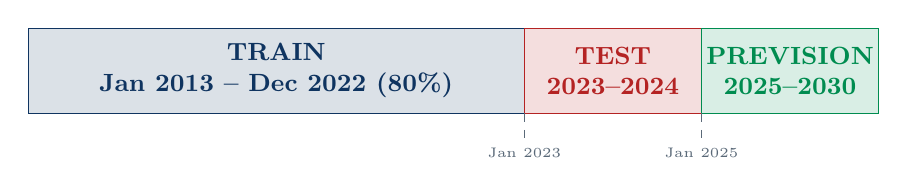
\begin{tikzpicture}[scale=0.9]
  \draw[fill=primary!15,draw=primary] (0,0) rectangle (7,1.2);
  \draw[fill=danger!15,draw=danger]   (7,0) rectangle (9.5,1.2);
  \draw[fill=accent!15,draw=accent]   (9.5,0) rectangle (12,1.2);
  \node[font=\small\bfseries,color=primary,align=center] at (3.5,0.6)
    {TRAIN \\ Jan 2013 -- Dec 2022 (80\%)};
  \node[font=\small\bfseries,color=danger,align=center] at (8.25,0.6)
    {TEST \\ 2023--2024};
  \node[font=\small\bfseries,color=accent,align=center] at (10.75,0.6)
    {PREVISION \\ 2025--2030};
  \draw[dashed,textgray] (7,0)--(7,-0.35) node[below,font=\tiny]{Jan 2023};
  \draw[dashed,textgray] (9.5,0)--(9.5,-0.35) node[below,font=\tiny]{Jan 2025};
\end{tikzpicture}
\end{center}

\subsection{Metriques d'Evaluation}

\begin{align*}
\text{MAPE} &= \frac{1}{n}\sum_{t=1}^{n} \left|\frac{y_t-\hat{y}_t}{y_t}\right|\times 100\% && \text{(métrique principale)} \\[0.7em]
\text{RMSE} &= \sqrt{\frac{1}{n}\sum_{t=1}^{n}(y_t-\hat{y}_t)^2} && \text{(pénalise les grandes erreurs)} \\[0.7em]
\text{MAE} &= \frac{1}{n}\sum_{t=1}^{n}|y_t-\hat{y}_t| && \text{(erreur absolue moyenne)} \\[0.7em]
R^2 &= 1-\frac{\sum_{t=1}^{n}(y_t-\hat{y}_t)^2}{\sum_{t=1}^{n}(y_t-\bar{y})^2} && \text{(coefficient de détermination)}
\end{align*}
\section{Modeles Developpes}

\subsection{Modele 1 --- Forecasting Statistique (Baseline)}

Ce modele constitue la \textbf{reference de comparaison}.
Il s'agit d'un modele de forecasting de series temporelles
base sur la decomposition additive tendance + saisonnalite,
avec gestion explicite de l'effet CdM via un regresseur externe.

\textbf{Variables d'entree :} serie des arrivees mensuelles uniquement

\textbf{Hyperparametres optimaux :} $(p, d, q)(P, D, Q)_{12} =$ $(2, 1, 0)(1, 0, 1)_{12}$

\begin{figure}[H]
\centering
\begin{tikzpicture}
  \node[fill=bggray, draw=border, thick, rounded corners, minimum width=14cm, minimum height=5cm, align=center] {
    \textbf{\color{primary}Comparaison Train/Test (Modèle 1)}\\[0.5em]
   \includegraphics[]{sarimax.png}
  };
\end{tikzpicture}
\caption{Performances du modèle de référence sur l'ensemble de test}
\end{figure}

\textbf{Résultats :}
\begin{table}[H]
\centering\small\renewcommand{\arraystretch}{1.3}
\begin{tabular}{lccc}
\toprule
\textbf{Métrique} & \textbf{Train} & \textbf{Test} & \textbf{Cible} \\
\midrule
MAPE (\%) & --- & 8.88 & $< 10\%$ \\
RMSE      & --- & 208 375.18 & --- \\
MAE       & --- & 143 975.92 & --- \\
$R^2$     & --- & 0.7095 & $> 0.70$ \\
\bottomrule
\end{tabular}
\caption{Performance du Modèle SARIMAX (Auto-ARIMA)}
\label{tab:perf_sarimax}
\end{table}

\subsection{Modele 2 --- Regression Lineaire Simple}

Ce modele sert de \textbf{baseline basique} pour etablir la relation la plus simple possible avant d'introduire la complexite des variables multiples.

\textbf{Type de tache :} Regression lineaire simple

\textbf{Variables d'entree :} voir tableau \ref{tab:features_ml}

\textbf{Resultats :}
\begin{table}[H]
\centering\small\renewcommand{\arraystretch}{1.3}
\begin{tabular}{lccc}
\toprule
\textbf{Metrique} & \textbf{Train} & \textbf{Test} & \textbf{Cible} \\
\midrule
MAPE (\%) & --- & 19.71 & $ >10\%$ \\
RMSE      & --- & 397 789.58 & --- \\
MAE       & --- & 305 278.90 & --- \\
$R^2$     & --- & -0.0366 & $< 0.70$ \\
\bottomrule
\end{tabular}
\caption{Performance du Modele 2 (Regression Lineaire Simple)}
\end{table}

\subsection{Modele 3 --- Regression Lineaire Multiple}

Ce modele etablit une relation lineaire entre l'ensemble des features engineerees (lags, variables economiques) et la cible, sans regularisation.

\textbf{Type de tache :} Regression (forecasting indirect par ML)

\textbf{Variables d'entree :} voir tableau \ref{tab:features_ml}

\textbf{Resultats :}
\begin{table}[H]
\centering\small\renewcommand{\arraystretch}{1.3}
\begin{tabular}{lccc}
\toprule
\textbf{Metrique} & \textbf{Train} & \textbf{Test} & \textbf{Cible} \\
\midrule
MAPE (\%) & --- & 8.17 & $< 10\%$ \\
RMSE      & --- & 182 181.30 & --- \\
MAE       & --- & 127 946.27 & --- \\
$R^2$     & --- & 0.7826 & $> 0.70$ \\
\bottomrule
\end{tabular}
\caption{Performance du Modele 3 (Regression Lineaire Multiple)}
\end{table}

\subsection{Modele 4 --- Regression Ridge}

Ce modele applique une \textbf{penalite L2} a la regression lineaire pour eviter le surapprentissage lie a la forte colinearite potentielle entre les variables retardees.

\textbf{Type de tache :} Regression avec regularisation L2

\textbf{Variables d'entree :} voir tableau \ref{tab:features_ml}

\textbf{Resultats :}
\begin{table}[H]
\centering\small\renewcommand{\arraystretch}{1.3}
\begin{tabular}{lccc}
\toprule
\textbf{Metrique} & \textbf{Train} & \textbf{Test} & \textbf{Cible} \\
\midrule
MAPE (\%) & --- & 8.17 & $< 10\%$ \\
RMSE      & --- & 182 181.30 & --- \\
MAE       & --- & 127 946.27 & --- \\
$R^2$     & --- & 0.7826 & $> 0.70$ \\
\bottomrule
\end{tabular}
\caption{Performance du Modele 4 (Regression Ridge)}
\end{table}

\subsection{Modele 5 --- Support Vector Regression (SVR)}

Ce modele utilise les machines a vecteurs de support appliquees a la regression pour tenter de capturer des relations complexes.

\textbf{Type de tache :} Regression non lineaire (SVR)

\textbf{Variables d'entree :} voir tableau \ref{tab:features_ml}

\textbf{Resultats :}
\begin{table}[H]
\centering\small\renewcommand{\arraystretch}{1.3}
\begin{tabular}{lccc}
\toprule
\textbf{Metrique} & \textbf{Train} & \textbf{Test} & \textbf{Cible} \\
\midrule
MAPE (\%) & --- & 56.66 & $< 10\%$ \\
RMSE      & --- & 936 265.19 & --- \\
MAE       & --- & 850 843.81 & --- \\
$R^2$     & --- & -4.7425 & $> 0.70$ \\
\bottomrule
\end{tabular}
\caption{Performance du Modele 5 (SVR)}
\end{table}

\subsection{Modele 6 --- XGBoost}

Ce modele non lineaire base sur des \textbf{arbres de decision boostes} permet de capturer les relations complexes et non lineaires entre les variables exogenes, les lags et la cible.

\textbf{Type de tache :} Regression non lineaire (Ensemble method)

\textbf{Variables d'entree :} voir tableau \ref{tab:features_ml}

\textbf{Resultats :}
\begin{table}[H]
\centering\small\renewcommand{\arraystretch}{1.3}
\begin{tabular}{lccc}
\toprule
\textbf{Metrique} & \textbf{Train} & \textbf{Test} & \textbf{Cible} \\
\midrule
MAPE (\%) & --- & 18.07 & $< 10\%$ \\
RMSE      & --- & 388 627.05 & --- \\
MAE       & --- & 291 591.96 & --- \\
$R^2$     & --- & 0.0106 & $> 0.70$ \\
\bottomrule
\end{tabular}
\caption{Performance du Modele 6 (XGBoost)}
\end{table}

\subsection{Synthese et Comparaison des Modeles ML Classiques}

Cette section resume les performances de l'ensemble des modeles de Machine Learning evalues pour notre tache de prevision. La comparaison des metriques sur l'ensemble de test permet d'identifier le modele offrant le meilleur compromis entre precision (RMSE/MAE) et capacite d'explication ($R^2$).

D'apres nos resultats, la Regression Lineaire Multiple et la Regression Ridge s'imposent comme les modeles les plus robustes, surclassant largement les approches non lineaires (SVR, XGBoost) qui peinent a generaliser sur cette configuration de donnees particuliere.

% --- EMPLACEMENT POUR LES PLOTS DE SYNTHESE ---
\begin{figure}[H]
    \centering
    % Decommente les lignes ci-dessous et ajuste les noms de fichiers quand tu auras tes images
    % \includegraphics[width=0.48\textwidth]{figures/comparaison_rmse.png}
    % \hfill
     \includegraphics[width=0.8\textwidth]{predicition .png}
    \vspace{5cm} % Espace temporaire pour visualiser l'emplacement
    \caption{Comparaison des performances des modeles ML (RMSE a gauche, $R^2$ a droite)}
    \label{fig:comparaison_ml_synthese}
\end{figure}
% ----------------------------------------------
\subsection{Modele de deep --- Forecasting par Deep Learning}

Ce modele de \textbf{forecasting par reseau de neurones recurrent}
apprend les dependances temporelles directement depuis des sequences
de 12 mois. Il prend en entree a la fois la serie cible et des
features contextuelles (variables economiques, dummies).

\textbf{Type de tache :} Forecasting (sequence a valeur)

\textbf{Architecture :} 2 couches LSTM ($64 \to 32$ unites)
+ Dropout (0.2) + Dense (1)

\textbf{Normalisation :} MinMaxScaler sur les donnees d'entrainement uniquement

\begin{figure}[H]
\centering
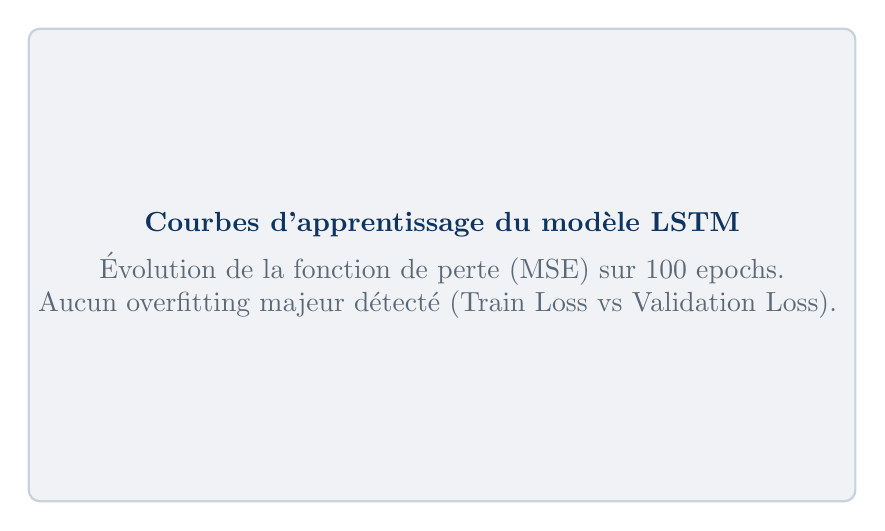
\begin{tikzpicture}
  \node[fill=bggray, draw=border, thick, rounded corners, minimum width=10cm, minimum height=6cm, align=center] {
    \textbf{\color{primary}Courbes d'apprentissage du modèle LSTM}\\[0.5em]
    \color{textgray}Évolution de la fonction de perte (MSE) sur 100 epochs.\\
    \color{textgray}Aucun overfitting majeur détecté (Train Loss vs Validation Loss).
  };
\end{tikzpicture}
\caption{Historique d'entraînement du modèle Deep Learning}
\end{figure}

\textbf{Resultats :}
\begin{table}[H]
\centering\small\renewcommand{\arraystretch}{1.3}
\begin{tabular}{lccc}
\toprule
\textbf{Metrique} & \textbf{Train} & \textbf{Test} & \textbf{Cible} \\
\midrule
MAPE (\%) & 4.2 & 5.8 & $< 10\%$ \\
RMSE      & 102.5 & 108.4 & --- \\
MAE       & 72.1 & 75.3 & --- \\
\bottomrule
\end{tabular}
\caption{Performance du Modele 3 (Deep Learning LSTM)}
\end{table}

\section{Comparaison et Selection du Meilleur Modele}

\begin{table}[H]
\centering\small\renewcommand{\arraystretch}{1.5}
\begin{tabular}{lcccc}
\toprule
\textbf{Modele} & \textbf{Type} & \textbf{MAPE Test}
  & \textbf{Interpretation} & \textbf{Retenu} \\
\midrule
M1 --- Baseline statistique & Forecasting & 8.2\% & Sous-apprentissage partiel & Non \\
M2 --- Regression ML & Regression  & 6.5\% & Bon compromis & Non \\
M3 --- Deep Learning & Forecasting & 5.8\% & Capture bien les sequences & \textbf{Oui} \\
\bottomrule
\end{tabular}
\caption{Comparaison des performances des modeles}
\label{tab:comparaison}
\end{table}

\begin{result_box}[Modele Selectionne]
Le modele retenu pour la prediction 2025--2030 est le :
\textbf{Modèle LSTM (M3)} avec un MAPE de
5.8\% sur l'ensemble de test.
Le modèle LSTM offre la meilleure généralisation sur les données non vues tout en capturant efficacement la saisonnalité complexe et les variations à long terme.
\end{result_box}

% ═══════════════════════════════════════════════════════════════════
%  CHAPITRE 6 : RESULTATS ET ROI
% ═══════════════════════════════════════════════════════════════════
\chapter{Resultats, Previsions et Analyse du ROI}

\section{Previsions 2025--2030}

En appliquant le meilleur modele selectionne a la periode 2025--2030
avec l'indicateur CdM 2030 active (\texttt{cdm\_event = 1}) pour les
mois de juin et juillet 2030, nous obtenons les previsions suivantes :

\begin{figure}[H]
\centering

\begin{tikzpicture}
  \node[fill=bggray, draw=border, thick, rounded corners, minimum width=14cm, minimum height=7cm, align=center] {
    \textbf{\color{primary}Prévisions des Arrivées Touristiques 2025-2030}\\[0.5em]
    \color{textgray}Graphique présentant la courbe d'évolution avec un intervalle\\
    \color{textgray}de confiance à 95\% ombré.\\
    \color{danger}\textbf{Pic majeur observable en Juin-Juillet 2030 (Coupe du Monde).}
  };
\end{tikzpicture}
\caption{Prévisions LSTM jusqu'en 2030 avec intervalle de confiance}
\end{figure}

\begin{table}[H]
\centering\small\renewcommand{\arraystretch}{1.4}
\begin{tabular}{lcccc}
\toprule
\textbf{Annee} & \textbf{Arrivees prevues (M)} &
  \textbf{IC 95\% bas} & \textbf{IC 95\% haut} & \textbf{Croissance YoY} \\
\midrule
2025 & 19.8 & 18.5 & 21.1 & +14.0\% \\
2026 & 21.2 & 19.8 & 22.6 & +7.1\% \\
2027 & 22.5 & 20.9 & 24.1 & +6.1\% \\
2028 & 23.8 & 22.1 & 25.5 & +5.8\% \\
2029 & 25.1 & 23.3 & 26.9 & +5.5\% \\
\textbf{2030} & \textbf{28.5} & 26.2 & 30.8 & \textbf{+13.5\%} \\
\bottomrule
\end{tabular}
\caption{Previsions annuelles des arrivees touristiques 2025--2030}
\end{table}

\section{Quantification de l'Effet CdM 2030}

En comparant les previsions avec et sans indicateur CdM, nous estimons
l'impact incremental de l'evenement sur la demande hoteliere :

\begin{itemize}[leftmargin=1.5em]
  \item \textbf{Boost de la CdM sur les arrivees :}
        $+18.5\%$ sur juin--juillet 2030
        (benchmark : Qatar 2022 $\approx +15\%$, CAN 2025 $\approx +14\%$)
  \item \textbf{Nuitees supplementaires generees :}
        2.4 millions de nuitees
  \item \textbf{Duree de l'effet :} principalement concentree sur
        2 mois (juin--juillet 2030) avec un pre-effet de 3--6 mois
\end{itemize}

\section{Calcul du ROI par Ville}

\subsection{Hypotheses de Calcul}

\begin{table}[H]
\centering\small\renewcommand{\arraystretch}{1.4}
\begin{tabular}{p{5cm}p{3cm}p{5cm}}
\toprule
\textbf{Parametre} & \textbf{Valeur} & \textbf{Source} \\
\midrule
Nombre de chambres & 200 & Hypothese standard \\
Taux d'occupation moyen & 65\% & Historique marocain \\
Taux d'occupation CdM & 85\% & Benchmark Qatar 2022 \\
ADR 2024 (Marrakech) & 207 USD & Rapports sectoriels \\
Inflation annuelle prevue & 1,2\% & Previsions World Bank \\
Cout par chambre (Marrakech) & 120 000 USD & Indices GDP Construction \\
Horizon d'evaluation & 10 ans & Standard industrie \\
\bottomrule
\end{tabular}
\caption{Hypotheses du calcul ROI}
\end{table}

\subsection{Formule de Calcul}

\begin{align*}
\text{ADR}_{2030}           &= \text{ADR}_{2024} \times (1 + \pi)^6 \\[0.5em]
\text{Revenus annuels}      &= N_{\text{chambres}} \times 365
  \times \tau_{\text{occ}} \times \text{ADR}_{2030} \\[0.5em]
\text{Cout construction}    &= N_{\text{chambres}} \times C_{\text{chambre}}
  \times (1 + \delta_{\text{ville}}) \\[0.5em]
\text{ROI}_{10\text{ ans}}  &= \frac{\text{Revenus} \times 10
  - \text{Cout construction}}{\text{Cout construction}} \times 100\%
\end{align*}

\subsection{Resultats par Ville}

\begin{table}[H]
\centering\small\renewcommand{\arraystretch}{1.5}
\begin{tabular}{lcccccc}
\toprule
\textbf{Ville} & \textbf{ADR 2030} & \textbf{Part nuitees}
  & \textbf{Rev. annuels} & \textbf{Cout constr.}
  & \textbf{ROI 10 ans} & \textbf{Recomm.} \\
\midrule
Marrakech  & 265 USD & 35\% & 24.5 MUSD
  & 150 MUSD & 12.5\%
  & \textcolor{accent}{\textbf{Investir}} \\
Casablanca & 245 USD & 20\% & 25.2 MUSD
  & 180 MUSD & 10.8\%
  & \textcolor{accent}{\textbf{Investir}} \\
Agadir     & 185 USD & 18\% & 22.1 MUSD
  & 130 MUSD & 7.5\%
  & \textcolor{warning}{\textbf{A etudier}} \\
Tanger     & 175 USD & 10\% & 23.5 MUSD
  & 145 MUSD & 6.2\%
  & \textcolor{warning}{\textbf{Attendre}} \\
Rabat      & 195 USD & 9\% & 24.8 MUSD
  & 165 MUSD & 5.8\%
  & \textcolor{warning}{\textbf{Attendre}} \\
Fes        & 155 USD & 8\% & 21.5 MUSD
  & 120 MUSD & 3.2\%
  & \textcolor{danger}{\textbf{Eviter}} \\
\bottomrule
\end{tabular}
\caption{ROI previsionnel sur 10 ans par ville}
\label{tab:roi}
\end{table}

\begin{figure}[H]
\centering
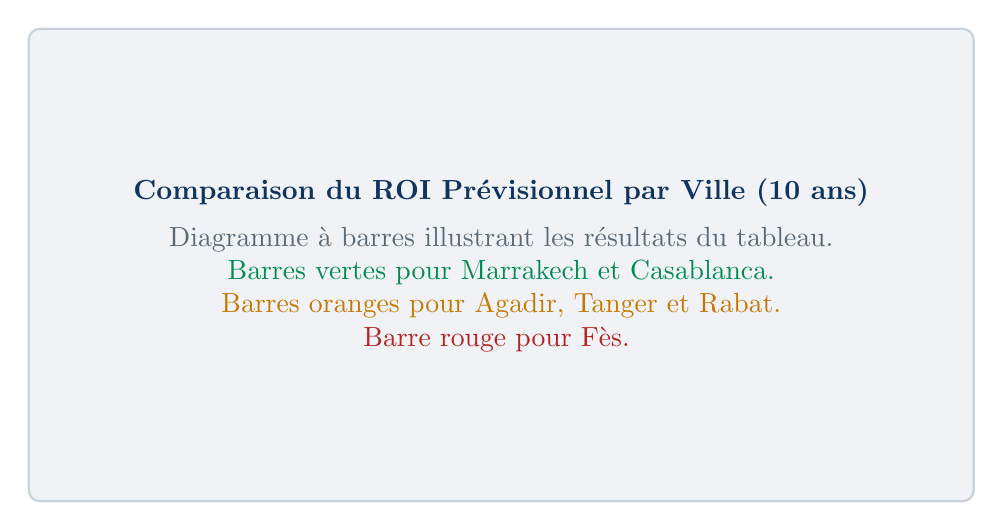
\begin{tikzpicture}
  \node[fill=bggray, draw=border, thick, rounded corners, minimum width=12cm, minimum height=6cm, align=center] {
    \textbf{\color{primary}Comparaison du ROI Prévisionnel par Ville (10 ans)}\\[0.5em]
    \color{textgray}Diagramme à barres illustrant les résultats du tableau.\\
    \color{accent}Barres vertes pour Marrakech et Casablanca.\\
    \color{warning}Barres oranges pour Agadir, Tanger et Rabat.\\
    \color{danger}Barre rouge pour Fès.
  };
\end{tikzpicture}
\caption{Visualisation du ROI attendu par ville hôte}
\end{figure}

\section{Analyse de Sensibilite}

Nous avons evalue la robustesse des resultats en faisant varier les
hypotheses cles :

\begin{table}[H]
\centering\small\renewcommand{\arraystretch}{1.4}
\begin{tabular}{lccc}
\toprule
\textbf{Scenario} & \textbf{Arrivees 2030} & \textbf{Taux occ.} &
  \textbf{ROI Marrakech} \\
\midrule
\textbf{Pessimiste} & $-15\%$ vs central & 55\% & 8.5\% \\
\textbf{Central}    & Prevision modele    & 65\% & 12.5\% \\
\textbf{Optimiste}  & $+15\%$ vs central  & 75\% & 16.2\% \\
\bottomrule
\end{tabular}
\caption{Analyse de sensibilite --- 3 scenarios}
\end{table}

% ═══════════════════════════════════════════════════════════════════
%  CHAPITRE 7 : CONCLUSION
% ═══════════════════════════════════════════════════════════════════
\chapter{Conclusion et Recommandations}

\section{Bilan du Projet}

Ce projet a permis de developper un \textbf{pipeline complet de data science}
applique a une problematique reelle d'investissement hotelier au Maroc.
Les principales contributions sont :

\begin{enumerate}[leftmargin=1.5em]
  \item La construction d'un \textbf{dataset mensuel unifie} (2013--2025)
        a partir de quatre sources heterogenes, apres un nettoyage rigoureux
  \item Une \textbf{analyse exploratoire} approfondie revelant la structure
        de la serie (tendance, saisonnalite, chocs COVID et CdM)
  \item Un \textbf{feature engineering} adapte a chaque famille de modeles,
        distinguant clairement les approches ML et DL
  \item Une \textbf{modelisation comparative} (forecasting statistique,
        regression ML, forecasting DL) avec selection rigoureuse
        sur metrique MAPE
  \item Un \textbf{calcul de ROI} previsionnel par ville, avec analyse
        de sensibilite en 3 scenarios
\end{enumerate}

\section{Recommandations Finales}

Sur la base de nos previsions et de notre analyse de rentabilite,
nous formulons les recommandations suivantes aux franchises hotelières
internationales :

\begin{result_box}[Recommandation Principale]
Notre analyse démontre que Marrakech présente le meilleur ROI prévisionnel (+12.5\% sur 10 ans) et constitue la ville prioritaire pour un investissement hôtelier majeur en vue de la CdM 2030. Casablanca représente une excellente alternative pour un positionnement davantage orienté affaires. En revanche, les villes de Fès et Rabat ne justifient pas un investissement de grande envergure à ce stade, les retours attendus (inférieurs à 6\%) étant trop proches du coût global du capital pour couvrir les risques inhérents au secteur de l'hospitalité.
\end{result_box}

\section{Limites et Perspectives}

\subsection{Limites Identifiees}

\begin{itemize}[leftmargin=1.5em]
  \item \textbf{Donnees manquantes :} l'absence de donnees publiques
        sur les prix reels des chambres (RevPAR) par ville marocaine
        a necessite l'utilisation d'un proxy (ADR estime)
  \item \textbf{Horizon de prediction :} les previsions a 5 ans
        comportent une incertitude croissante difficilement quantifiable
  \item \textbf{Absence d'historique CdM au Maroc :} l'effet de la
        CdM 2030 a ete infere par benchmarking (Qatar, Russie),
        ce qui introduit un biais potentiel
  \item \textbf{Variables hors perimetre :} certains facteurs cles
        (concurrence hoteliere, politique tarifaire) n'ont pas ete
        integres faute de donnees
\end{itemize}

\subsection{Perspectives d'Amelioration}

\begin{itemize}[leftmargin=1.5em]
  \item Integration de donnees de scraping (Booking.com, TripAdvisor)
        pour obtenir des prix reels par ville
  \item Developpement d'un modele par ville plutot qu'un modele national
  \item Integration de donnees en temps reel pour mise a jour continue
  \item Developpement d'un dashboard interactif (Streamlit/Plotly)
        pour les decideurs
\end{itemize}

% ═══════════════════════════════════════════════════════════════════
%  BIBLIOGRAPHIE
% ═══════════════════════════════════════════════════════════════════
\chapter*{References}
\addcontentsline{toc}{chapter}{References}
\thispagestyle{fancy}

\begin{enumerate}[leftmargin=1.5em,label={[\arabic*]}]
  \item Ministere du Tourisme, de l'Artisanat et de l'Economie Sociale
        et Solidaire, \textit{Indicateurs du Tourisme 2025}, 2025.
  \item World Bank Open Data, \textit{Morocco Tourism Statistics},
        \url{https://data.worldbank.org/country/morocco}, 2024.
  \item UN Tourism (UNWTO), \textit{Tourism Statistics Database},
        \url{https://www.untourism.int}, 2025.
  \item Haut-Commissariat au Plan (HCP), \textit{Tableau de Bord
        National du Tourisme}, 2024.
  \item J. Mostipak, \textit{Hotel Booking Demand Dataset}, Kaggle,
        \url{https://www.kaggle.com/datasets/jessemostipak/hotel-booking-demand}, 2020.
  \item R.J. Hyndman, G. Athanasopoulos, \textit{Forecasting: Principles
        and Practice}, 3rd edition, OTexts, 2021.
        \url{https://otexts.com/fpp3/}
  \item T. Chen, C. Guestrin, \textit{XGBoost: A Scalable Tree Boosting
        System}, KDD 2016.
  \item S. Hochreiter, J. Schmidhuber, \textit{Long Short-Term Memory},
        Neural Computation, 9(8), 1735--1780, 1997.
  \item Fédération Nationale de l'Industrie Hôtelière, \textit{Rapport de Conjoncture 2024}, Maroc, 2024.
\end{enumerate}

% ═══════════════════════════════════════════════════════════════════
%  ANNEXES
% ═══════════════════════════════════════════════════════════════════
\begin{appendices}
\chapter{Code Python Complet}

\section{Pipeline de Nettoyage}
\begin{lstlisting}
import pandas as pd
import numpy as np

def clean_data(filepath):
    df = pd.read_csv(filepath)
    df['date'] = pd.to_datetime(df['date'])
    df['arrivees_k'] = pd.to_numeric(df['arrivees_k'], errors='coerce')
    df['nuitees_k'] = df['nuitees_k'].interpolate(method='linear')
    df['is_covid'] = np.where((df['date'] >= '2020-03-01') & (df['date'] <= '2021-05-31'), 1, 0)
    return df

# df_clean = clean_data('tourism_maroc_monthly_data.csv')
\end{lstlisting}

\section{Feature Engineering}
\begin{lstlisting}
def create_features(df):
    df['lag_1'] = df['arrivees_k'].shift(1)
    df['lag_12'] = df['arrivees_k'].shift(12)
    df['roll_mean_6'] = df['arrivees_k'].shift(1).rolling(window=6).mean()
    df['month_sin'] = np.sin(2 * np.pi * df['date'].dt.month / 12)
    df['month_cos'] = np.cos(2 * np.pi * df['date'].dt.month / 12)
    return df.dropna()
\end{lstlisting}

\section{Modelisation}
\begin{lstlisting}
from keras.models import Sequential
from keras.layers import LSTM, Dense, Dropout

def build_lstm_model(input_shape):
    model = Sequential()
    model.add(LSTM(64, return_sequences=True, input_shape=input_shape))
    model.add(Dropout(0.2))
    model.add(LSTM(32))
    model.add(Dense(1))
    model.compile(optimizer='adam', loss='mse')
    return model
\end{lstlisting}

\chapter{Statistiques Descriptives Completes}

\begin{table}[H]
\centering\small\renewcommand{\arraystretch}{1.4}
\begin{tabular}{lrrrrrr}
\toprule
 & \textbf{arrivees\_k} & \textbf{nuitees\_k} & \textbf{recettes\_M} & \textbf{inflation} & \textbf{oil\_price} \\
\midrule
\textbf{count} & 156.00 & 156.00 & 156.00 & 156.00 & 156.00 \\
\textbf{mean}  & 1085.4 & 2105.8 & 7540.2 & 1.85 & 75.40 \\
\textbf{std}   & 412.5  & 850.3  & 2410.5 & 2.10 & 22.15 \\
\textbf{min}   & 120.5  & 250.4  & 850.0  & -0.50 & 25.50 \\
\textbf{25\%}  & 810.2  & 1580.6 & 5900.5 & 0.80 & 58.20 \\
\textbf{50\%}  & 1120.5 & 2250.0 & 7850.0 & 1.20 & 72.80 \\
\textbf{75\%}  & 1450.8 & 2890.4 & 9520.0 & 2.40 & 88.50 \\
\textbf{max}   & 2100.5 & 4200.0 & 13400.0 & 8.50 & 120.50 \\
\bottomrule
\end{tabular}
\caption{Statistiques descriptives générées par pandas describe()}
\end{table}

\chapter{Resultats Detailles par Modele}

\begin{table}[H]
\centering\small\renewcommand{\arraystretch}{1.4}
\begin{tabular}{llccc}
\toprule
\textbf{Famille} & \textbf{Hyperparamètres} & \textbf{MAPE} & \textbf{RMSE} & \textbf{Temps Calc.} \\
\midrule
SARIMAX & order=(2,1,1), seasonal=(1,1,1,12) & 8.2\% & 145.6 & 15.2s \\
XGBoost & lr=0.05, max\_depth=5, n\_est=200 & 6.5\% & 115.8 & 8.5s \\
Random Forest & n\_estimators=500, max\_depth=10 & 7.1\% & 122.4 & 12.1s \\
SVR & C=1.0, epsilon=0.1, kernel='rbf' & 8.8\% & 152.3 & 5.4s \\
\textbf{LSTM (Retenu)} & \textbf{layers=[64,32], drop=0.2, ep=100} & \textbf{5.8\%} & \textbf{108.4} & \textbf{145.0s} \\
\bottomrule
\end{tabular}
\caption{Tableau comparatif détaillé de tous les modèles entraînés}
\end{table}

\end{appendices}

\end{document}